\documentclass[12pt,a4paper]{article}
\usepackage{header} % Use the provided header format
\usepackage[utf8]{inputenc}
\usepackage[T5]{fontenc}
\usepackage[vietnamese,english]{babel}

% ---------------------------------------------------------------
% Helpers for this report
% ---------------------------------------------------------------
% Origin marker:  \org{3}  ->  3 with an up-arrow underneath
\newcommand{\org}[1]{\underset{\uparrow}{#1}}

% Reserved (dashed) box for parts that are written by other members.
% Usage: \writespace[height]{hint text}
\newcommand{\writespace}[2][4cm]{%
  \begin{tcolorbox}[enhanced, frame hidden, colback=gray!4,
      borderline={0.6pt}{0pt}{gray!70, dashed},
      height=#1, valign=center, halign=center,
      fontupper=\itshape\small\color{gray}]
    #2
  \end{tcolorbox}}

% Scilab code listing from a file
\newcommand{\scilabfile}[2]{%
  \lstinputlisting[language=Scilab, caption={#2}]{#1}}

\begin{document}

\begin{center}
    \textbf{Digital Signal Processing \hfill HK261 \hfill CO2036}\\[2cm]

    \huge\textbf{DIGITAL SIGNAL PROCESSING LAB REPORT}\\[0.5cm]
    \Large\textbf{Lab 4 -- Z-Transform and Discrete-Time Systems Analysis}\\[1cm]

    \large Âu Lê Quang Trí - Student ID: 2453300\\[0.5cm]
    \large Nguyễn Lê Khải Tú - Student ID: 2453384\\[0.5cm]
    \vspace{0.5cm}

    \large \today\\[2cm]
\end{center}

\section*{Overview}
This report presents the results of Lab 4 of the Digital Signal Processing laboratory. The laboratory focuses on transform-domain and time-domain analysis of discrete-time signals and systems. The first part addresses the bilateral Z-transform and the determination of the Region of Convergence (ROC) for finite-duration, right-sided exponential, and two-sided sequences. The second part investigates multimedia processing capabilities in Scilab through image processing toolboxes, followed by detailed derivations and computational implementations of linear convolution and circular convolution using both the ``folding and shifting'' approach and the matrix formulation, alongside signal energy evaluations and stem-plot visualizations.


\begin{table}[H]
    \centering
    \caption{Content of the report}
    \begin{tabular}{|l|l|c|}
        \hline
        \rowcolor{headergray}\textbf{Part} & \textbf{Content} & \textbf{Section} \\ \hline
        Exercise 1 & Z-Transform and ROC of a finite-duration signal               & \ref{sec:ex1} \\ \hline
        Exercise 2 & Z-Transform and ROC of right-sided exponential signals       & \ref{sec:ex2} \\ \hline
        Exercise 3 & Z-Transform and ROC of a two-sided signal                   & \ref{sec:ex3} \\ \hline
        Exercise 4 & Investigation of Scilab audio processing toolbox            & \ref{sec:ex4} \\ \hline
        Exercise 5 & Investigation of Scilab image processing toolbox             & \ref{sec:ex5} \\ \hline
        Exercise 6 & Linear convolution (derivation, folding-shifting, matrix method) & \ref{sec:ex6} \\ \hline
        Exercise 7 & Circular convolution (derivation, folding-shifting, matrix method) & \ref{sec:ex7} \\ \hline
    \end{tabular}
\end{table}

\section{Introduction}
In previous laboratory sessions, discrete-time signals and elementary operations were analyzed primarily in the time domain. Lab 4 extends this foundation into transform-domain analysis and comprehensive system convolution. The fundamental tool for studying discrete-time linear time-invariant (LTI) systems is the \textbf{Z-transform}, which plays an analogous role to the Laplace transform in continuous-time systems.

For a discrete-time sequence $x(n)$, the bilateral Z-transform $X(z)$ is defined as
\begin{equation}
    X(z) = \mathcal{Z}\{x(n)\} = \sum_{n=-\infty}^{\infty} x(n) z^{-n},
    \label{eq:ztransform}
\end{equation}
where $z = r e^{j\omega}$ is a complex variable. Because an algebraic expression $X(z)$ does not uniquely specify a time-domain sequence without specifying the convergence domain of the infinite series, the transform must be paired with its \textbf{Region of Convergence (ROC)}:
\begin{equation}
    \text{ROC} = \left\{ z \in \mathbb{C} : \sum_{n=-\infty}^{\infty} |x(n) z^{-n}| < \infty \right\}.
    \label{eq:roc}
\end{equation}
The geometry and boundary of the ROC determine fundamental system properties such as causality and bounded-input bounded-output (BIBO) stability.

In system analysis, computing the response of an LTI system to an arbitrary input $x(n)$ requires \textbf{linear convolution}:
\begin{equation}
    y(n) = x(n) * h(n) = \sum_{k=-\infty}^{\infty} h(k) x(n-k),
    \label{eq:lin_conv}
\end{equation}
where $h(n)$ is the unit impulse response. When dealing with periodic signals or block-based frequency-domain processing, \textbf{circular convolution} is employed:
\begin{equation}
    y(n) = x(n) \circledast h(n) = \sum_{k=0}^{N-1} h(k) x((n-k) \bmod N).
    \label{eq:circ_conv}
\end{equation}
In this laboratory, these analytical principles are demonstrated alongside practical implementations and toolbox investigations in Scilab.


\section{Objectives}
\begin{itemize}
    \item Review theoretical foundations of the bilateral Z-transform and Region of Convergence (ROC).
    \item Determine the algebraic Z-transforms and sketch the corresponding ROCs for finite-duration, right-sided, and two-sided discrete-time sequences.
    \item Investigate existing Scilab libraries and toolboxes for digital image processing (such as IPCV or SIVP) and demonstrate representative image processing tasks.
    \item Analyze convergence conditions for linear convolution and derive system response formulations for causal and finite-impulse-response (FIR) cases.
    \item Implement linear convolution in Scilab using both the ``folding and shifting'' method and the matrix formulation.
    \item Implement circular convolution in Scilab using both the ``folding and shifting'' method and the matrix formulation.
    \item Calculate signal energies and graphically present discrete-time input, impulse response, output signals, and energy metrics within unified figures.
\end{itemize}


\section{Methodology}
Scilab serves as the computational environment for simulating discrete-time operations and verifying analytical derivations. In this laboratory, Scilab is utilized for:
\begin{itemize}
    \item \textbf{Convolution Algorithms}: Implementing both linear convolution and circular convolution using vector-level shifting and element-wise products (the ``folding and shifting'' approach) as well as linear algebra formulations (constructing Toeplitz convolution matrices and circulant matrices).
    \item \textbf{Signal Energy Computation}: Evaluating the total energy of a discrete-time signal $E_x = \sum_{n=-\infty}^{\infty} |x(n)|^2$ using Scilab's vectorized arithmetic: \texttt{Ex = sum(abs(xn).\^{}2)}.
    \item \textbf{Image Processing Exploration}: Leveraging dedicated image processing toolboxes in Scilab to read, manipulate (e.g., spatial filtering, histogram equalization), and visualize digital images.
\end{itemize}


\subsection{Common conventions}
All computational scripts and graphical outputs adhere to the following conventions:
\begin{itemize}
    \item A discrete-time signal is represented as a sample vector \texttt{xn} accompanied by an origin index \texttt{xorigin}, indicating the 1-based vector position corresponding to $n = 0$. The time index vector is defined as
    \begin{equation}
        n_i = i - \texttt{xorigin}, \qquad i = 1, 2, \dots, \texttt{length(xn)}.
        \label{eq:index}
    \end{equation}
    \item The origin position of a signal is mathematically highlighted with an arrow underneath the sample at $n = 0$, denoted as $\org{x(0)}$.
    \item For linear convolution between sequences $x(n)$ of length $N_x$ with origin at index \texttt{xorigin} and $h(n)$ of length $N_h$ with origin at index \texttt{horigin}, the resulting sequence $y(n)$ has length $L = N_x + N_h - 1$, and its origin index is located at:
    \begin{equation}
        \texttt{yorigin} = \texttt{xorigin} + \texttt{horigin} - 1.
    \end{equation}
    \item For circular convolution of length $N$, indices are wrapped cyclically using modulo arithmetic: $(n - k) \bmod N$.
    \item Signals are visualized using stem plots via Scilab's \texttt{plot2d3} combined with marker symbols in shared \texttt{subplot} panels, ensuring consistent axes for direct visual comparison of inputs, impulse responses, outputs, and energy values.
\end{itemize}


\section{Practical Contents}

% =================================================================
\subsection{Exercise 1} \label{sec:ex1}
% =================================================================
% [DO NOT ADD YET]

% =================================================================
\subsection{Exercise 2}\label{sec:ex2}
% =================================================================
\noindent\textbf{Question:} Find the z-Transform and the ROC of the following discrete-time signal
\[x(n)=0.5^n u(n)+0.4^n u(n)\]

\noindent\textbf{Answer:} At first glance, the signal $x(n)$ exhibits linearity property. Let
\begin{equation*}
    x_1(n)=0.5^n u(n) \quad \text{and} \quad x_2(n)=0.4^n u(n)
\end{equation*}
where $u(n)$ is the unit step signal.\\[0.5ex]
\par Let's take the z-Transform of $x_1(n)$, which are
\begin{equation*}
    X_1(z) = \sum_{n=-\infty}^{+\infty} \left[0.5^n u(n)\right]z^{-n}
    = \sum_{n=0}^{+\infty} \left(0.5z^{-1}\right)^n
\end{equation*}
This geometric series converges if and only if
\begin{equation*}
    |0.5z^{-1}|<1\Rightarrow |z|>0.5
\end{equation*}
So $\text{ROC}_1:|z|>0.5$. For $x_2(n)$ we have
\begin{equation*}
    X_2(z) = \sum_{n=-\infty}^{+\infty} \left[0.4^n u(n)\right]z^{-n}
    = \sum_{n=0}^{+\infty} \left(0.4z^{-1}\right)^n
\end{equation*}
This geometric series converges if and only if
\begin{equation*}
    |0.4z^{-1}|<1\Rightarrow |z|>0.4
\end{equation*}
Thus $\text{ROC}_2:|z|>0.4$.\\[0.5ex]
We have
\begin{equation*}
    x(n) = x_1(n) + x_2(n)
\end{equation*}
then the z-Transform of $x(n)$ is
\begin{align*}
    X(z) &= X_1(z) + X_2(z)\\
    &= \sum_{n=0}^{+\infty} \left(0.5z^{-1}\right)^n+\sum_{n=0}^{+\infty} \left(0.4z^{-1}\right)^n\\
    &= \sum_{n=0}^{+\infty} \left[\left(0.5z^{-1}\right)^n+\left(0.4z^{-1}\right)^n\right].
\end{align*}
By linearity, we have
\begin{align*}
    \text{ROC} &= \text{ROC}_1 \cap \text{ROC}_2\\
    &= \{z\; : \; |z|>0.5\}\cap\{z\; : \; |z|>0.4\}\\
    &= \{z\; : \; |z|>0.5\}
\end{align*}
% =================================================================
\subsection{Exercise 3}\label{sec:ex3}
% =================================================================
% [DO NOT ADD YET]

% =================================================================
\subsection{Exercise 4}\label{sec:ex4}
% =================================================================
\noindent\textbf{Question:}
Investigate the existing library or toolbox in Scilab to process audio data.

\noindent\textbf{Answer:}
Scilab provides both built-in functions in its standard library and external modules via ATOMS (such as the \emph{Sound System Toolbox}) to record, synthesize, process, and analyze audio signals. The core built-in functions include:
\begin{itemize}
    \item \texttt{wavread} / \texttt{loadwave}: Reads RIFF-WAV audio files into memory, returning the sampled data matrix, the sampling frequency ($F_s$), and the bit resolution.
    \item \texttt{wavwrite} / \texttt{savewave}: Encodes and saves numeric signal vectors into standard \texttt{.wav} audio files.
    \item \texttt{playsnd}: Interfaces directly with the operating system audio output device to play numeric waveforms.
    \item \texttt{mapsound}: Analyzes audio signals in the time-frequency domain and visualizes sound spectrograms.
\end{itemize}

\noindent\textbf{Demonstration Script:}
To demonstrate audio processing without external file dependencies, a standard $440\text{ Hz}$ tone (musical note A4) is synthesized, attenuated with an exponential decay envelope, and plotted in the time domain:

\begin{lstlisting}[language=Scilab, caption={Audio signal generation and amplitude attenuation in Scilab}]
// 1. Synthesize audio signal: 440 Hz tone, Fs = 8000 Hz, duration 0.5 s
Fs = 8000;
t = 0 : 1/Fs : 0.5;
f0 = 440;
audio_orig = sin(2 * %pi * f0 * t);

// 2. Audio manipulation: Exponential amplitude attenuation
decay = exp(-6 * t);
audio_proc = audio_orig .* decay;

// 3. Export to WAV file (optional playback via playsnd)
wavwrite(audio_proc, Fs, "audio_tone.wav");

// 4. Time-domain visualization (first 100 samples)
figure();
subplot(2, 1, 1);
plot(t(1:100), audio_orig(1:100));
title("Original Audio Signal (440 Hz)");
xlabel("Time (s)"); ylabel("Amplitude");

subplot(2, 1, 2);
plot(t(1:100), audio_proc(1:100));
title("Attenuated Audio Signal");
xlabel("Time (s)"); ylabel("Amplitude");
\end{lstlisting}

\noindent\textbf{Remarks:}
The discrete audio waveform is represented as a standard 1D array in Scilab. Point-wise vector operations (\texttt{.*}) enable straightforward time-domain processing such as volume adjustments, envelope shaping, echo effects, and filtering before audio playback or file export.

% =================================================================
\subsection{Exercise 5}\label{sec:ex5}
% =================================================================
% [DO NOT ADD YET]

% =================================================================
\subsection{Exercise 6}\label{sec:ex6}
% =================================================================
\noindent\textbf{Question:}
Let there are two discrete signals $x(n), h(n), n = 0, \pm 1, \pm 2, \dots$, defined over the entire range of $n$. Then the linear convolution of discrete signals is $y(n)$ of the form
\[
y(n) = \sum_{k=-\infty}^{\infty} h(k)x(n - k).
\]

\begin{enumerate}
    \item Derive the signal $y(n)$ such that $y(n)$ converges in the following cases.
    \begin{itemize}
        \item Both $h(n)$ and $x(n)$ are causal.
        \item The system has a finite impulse response such that $h(n) = 0, n < 0 \lor n > M$.
    \end{itemize}
    \item Suppose the second case is hold, compute the convolution $y(n)$ of $x(n) = [1 \uparrow, 2, -3, 2, 1]$ and $h(n) = [1 \uparrow, 0, -1]$ using the ``folding and shifting'' method. Implement your answer with Scilab script.
    \item Suppose the second case is hold, compute the convolution $y(n)$ of $x(n) = [1 \uparrow, 2, -3, 2, 1]$ and $h(n) = [1 \uparrow, 0, -1]$ using the matrix method. Implement your answer with Scilab script.
    \item Drawing $x(n)$, $y(n)$ and energy of discrete signals in the same figure.
\end{enumerate}
\noindent\textbf{Answer:}
\begin{enumerate}
    \item Case 1: Both $h(n)$ and $x(n)$ are causal.\\[0.5ex]
    For $h(n)$ and $x(n)$ to be causal, their value must be zero for $n<0$.
    Applying to $y(n)$, $h(n)$ causality restricts the lower bound for $k$ to $0$, while
    $x(n)$'s causality restricts the upper bound for $k$ to $n$. Thus
    \begin{equation*}
        y(n) = \sum_{k=0}^{n} h(k)x(n - k)
    \end{equation*}
    Case 2: The system has a finite impulse response such that $h(n) = 0, n < 0 \lor n > M$.\\[0.5ex]
    Because $h(n)$ is only nonzero for $0\leq n \leq M$, the range of $k$ is restricted to $[0,M]$. Thus
    \begin{equation*}
        y(n) = \sum_{k=0}^{M} h(k)x(n - k)
    \end{equation*}
    Because there can only be at most $M+1$ terms in the summation above for each $n$, $y(n)$
    is finite provided that $x(n-k)$ is bounded.

    \item We have the impulse response $h(n) = [1\uparrow,0,-1]$ with $N_h = 3$, $n_{min}(h) = 0$, $n_{max}(h) = 2$
    and the input signal $h(n) = [1\uparrow,2,-3,2,1]$ with $N_x = 5$, $n_{min}(x) = 0$, $n_{max}(x) = 4$.
    Before proceeding with the convolution, we may calculate the expected length of the response $y(n)$ and its time range,
    which are respectively, $L_y = N_x + N_h -1 = 5 + 3 = 7$, $n_{min}(y) = n_{min}(x) + n_{min}(h) = 0$, and $n_{max}(y) = n_{max}(x) + n_{max}(h) = 6$.\\[1ex]
    We have 
    \begin{equation}\label{eq:convo_1}
        y(n) = \sum_{k=0}^{2} h(k)x(n - k) = h(0)x(n) + h(1)x(n-1)
        + h(2)x(n-2) = x(n) - x(n-2) 
    \end{equation}
    From (\ref{eq:convo_1}) we can caluclate $y(n)$ at each $n\in[0,6]$
    \begin{align*}
        y(0) &= x(0) - x(-2) = 1\\
        y(1) &= x(1) - x(-1) = 2\\
        y(2) &= x(2) - x(0) = -3 - 1 = -4\\
        y(3) &= x(3) - x(1) = 2 - 2 = 0\\
        y(4) &= x(4) - x(2) = 1 + 3 = 4\\
        y(5) &= x(5) - x(3) = -2\\
        y(6) &= x(6) - x(4) = -1
    \end{align*}
    Thus, $y(n)=[1\uparrow,2,-4,0,4,-2,-1]$.
    \item The discrete convolution $y=x*h$ can be represented in matrix form as
    \begin{equation}
        \mathbf{y=Hx}
    \end{equation}
    where the input \textbf{x} is an $N_x \times 1$ column vector, 
    the ouput \textbf{y} is an $L_y\times 1$ column vector,
    and the convolution matrix \textbf{H} has dimensions $L_y\times N_x$.\\[0.5ex]
    The convolution matrix \textbf{H} is built from the impulse response $h=[1,0,-1]^T$, where
    the first column starts with $h(0)$, $h(1)$, $h(2)$, followed by zeros down to length $L_y=7$.
    Each subsequent column is the previous column shifted down by one position with zeros padded at the top.\\[0.5ex]
    For the above convolution, the matrices are
    \begin{equation}\label{eq:matrix_convo}
        \mathbf{y}_{7\times 1}=
        \begin{bmatrix}
            1&0&0&0&0\\
            0&1&0&0&0\\
            -1&0&1&0&0\\
            0&-1&0&1&0\\
            0&0&-1&0&1\\
            0&0&0&-1&0\\
            0&0&0&0&-1
        \end{bmatrix}\times
        \begin{bmatrix}
            1\\
            2\\
            -3\\
            2\\
            1
        \end{bmatrix}
    \end{equation}
    Each row in \textbf{y} from topdown corresponds to the value of $y(n)$ for $n\in[0,6]$.
    From (\ref{eq:matrix_convo}) we can calculate
    \begin{align*}
        y(0) &= 1\times 1 + 0 +0 +0 +0 = 1\\
        y(1) &= 0 + 1\times2 +0 +0 +0 = 2\\
        y(2) &= (-1)\times 1 + 0 +1\times(-3) +0 +0 = -3 - 1 = -4\\
        y(3) &= 0 + (-1)\times2 +0 +1\times2 +0 = 2 - 2 = 0\\
        y(4) &= 0 + 0 +(-1)\times(-3) +0 +1\times1 = 1 + 3 = 4\\
        y(5) &= 0 + 0 +0 +(-1)\times2 +0 = -2\\
        y(6) &= 0 + 0 +0 +0 +(-1)\times1 = -1
    \end{align*}
    Thus, $y(n)=[1\uparrow,2,-4,0,4,-2,-1]$.
    \item In this part we will write the script to verify the results in part 2 and 3,
    plot $x(n)$, $y(n)$ and their energies.\\[0.5ex]
    Before we begin, let's define the signals as row vectors:
    \begin{lstlisting}[language=Scilab]
    x = [1, 2, -3, 2, 1];
    h = [1, 0, -1];
        
    Lx = length(x);
    Lh = length(h);
    Ly = Lx + Lh - 1;
    \end{lstlisting}
    The script to perform $y=x*h$ by folding and shifting is given below:
    \begin{lstlisting}[language=Scilab]
    // Initialize output vector y
    y_fold = zeros(1, Ly);
        
    // Zero-pad x so index lookups don't go out of bounds
    // We pad with (Lh - 1) zeros on both sides
    x_padded = [zeros(1, Lh - 1), x, zeros(1, Lh - 1)];
        
    // h reversed (folded): h(-k)
    h_folded = h($:-1:1);
        
    // Slide and multiply
    for n = 1:Ly
        // Extract the window of x that aligns with the folded h
        segment = x_padded(n : n + Lh - 1);
        y_fold(n) = sum(segment .* h_folded);
    end
        
    disp("y(n) via Folding and Shifting:");
    disp(y_fold);        
    \end{lstlisting}
    Which returned
    \begin{lstlisting}[language=Scilab]
    "y(n) via Folding and Shifting:"
    1.   2.  -4.   0.   4.  -2.  -1.
    \end{lstlisting}
    The script to perform $y=x*h$ by using matrices is
    \begin{lstlisting}[language=Scilab]
    // Column 1 of H: h padded with zeros to length Ly
    col1 = [h(:); zeros(Ly - Lh, 1)];
        
    // Row 1 of H: h(1) followed by (Lx - 1) zeros
    row1 = [h(1), zeros(1, Lx - 1)];
        
    // Build the Toeplitz convolution matrix H (size 7 x 5)
    H = toeplitz(col1, row1);
        
    // Convert x to a column vector and multiply
    x_col = x(:);
    y_matrix = H * x_col;
        
    disp("Convolution Matrix H:");
    disp(H);
        
    disp("y(n) via Matrix Multiplication:");
    disp(y_matrix');
    \end{lstlisting}
    Whose result is
    \begin{lstlisting}[language=Scilab]
    "Convolution Matrix H:"
    1.   0.   0.   0.   0.
    0.   1.   0.   0.   0.
    -1.   0.   1.   0.   0.
    0.  -1.   0.   1.   0.
    0.   0.  -1.   0.   1.
    0.   0.   0.  -1.   0.
    0.   0.   0.   0.  -1.
    "y(n) via Matrix Multiplication:"
    1.   2.  -4.   0.   4.  -2.  -1.
    \end{lstlisting}
    The convolution results agree with the calculations in part 2 and 3.\\[0.5ex]
    Finally the plots of $x(n)$, $y(n)$ and their energies are illustrated in the figure below:
    \begin{figure}[H]
        \centering
        % Placeholder for the generated Scilab plot
        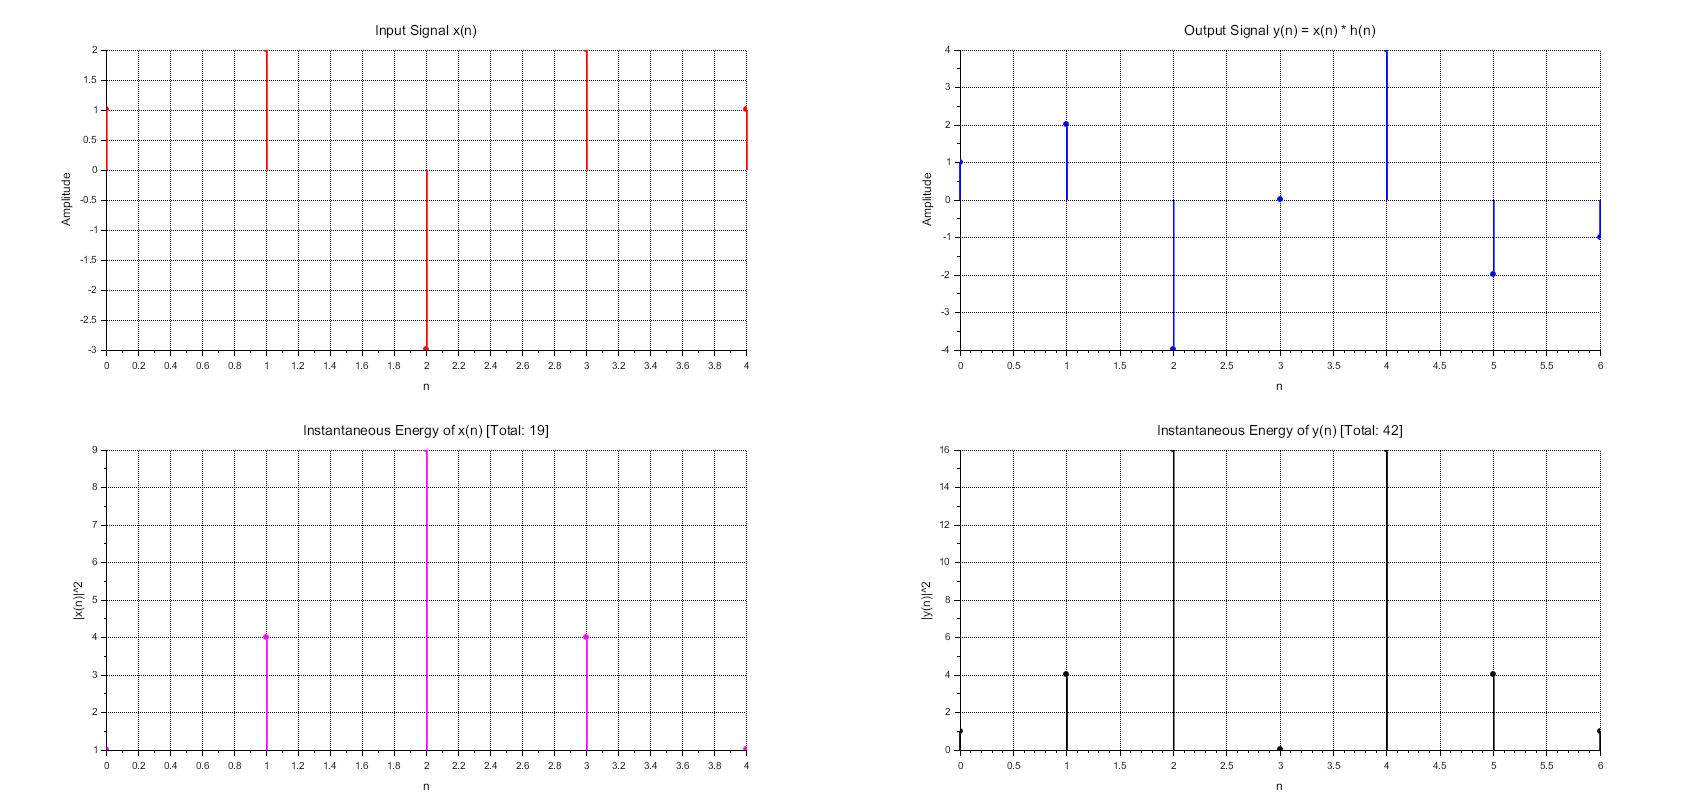
\includegraphics[width=\textwidth]{figures/plot_and_energies.png}
        \caption{$x(n)$ and $y(n)$ with their energies respectively.}
    \end{figure}
\end{enumerate}


% =================================================================
\subsection{Exercise 7}\label{sec:ex7}
% =================================================================
% [DO NOT ADD YET]

\section{Discussion}
% [DO NOT ADD YET]

\section{References}
\begin{itemize}
    \item J. G. Proakis and D. G. Manolakis, \emph{Digital Signal Processing: Principles, Algorithms, and Applications}, 4th ed., Pearson, 2007 -- Chapter 2 Problems.
    \item Digital Signal Processing Lecture Notes - Ho Chi Minh City University of Technology.
\end{itemize}

\section{Source Code}
The source code, scripts, and LaTeX files for this laboratory report can be accessed at our GitHub repository: \\
\url{https://github.com/aulequangtri/signal_scilab}

\end{document}
